\documentclass[10pt,a4paper]{article}
\author{Jannik Koch}
\title{Computergrafik}

\usepackage[utf8]{inputenc}
\usepackage[ngerman]{babel}
\usepackage{multicol}
\usepackage{amsmath}
\usepackage[a4paper, total={6in, 8in}]{geometry}
\usepackage{mathrsfs}
\usepackage{hyperref}
\usepackage{graphicx}
\usepackage{tikz}
\usepackage{pgfplots}

\graphicspath{{./images/}}

\def\realnumbers{{\rm I\!R}}
\def\polynomials{{\rm I\!P}}

\newcommand{\rom}[1]{\uppercase\expandafter{\romannumeral #1\relax}}
\newcommand{\norm}[1]{\lVert#1\rVert}
\renewcommand{\arraystretch}{1.5}
\setlength{\parindent}{0cm}

\begin{document}
	\pagenumbering{Roman}
	{\let\newpage\relax\maketitle}
	\tableofcontents
	\newpage
	\pagenumbering{arabic}
	\setcounter{page}{1}

	\section{Bilder, Farbe, Perzeption}
	\label{bfp:sec:bilder_farbe_perzeption}
	
	\subsection{Rasterbilder}
	\label{bfp:sub:rasterbilder}

	Rasterbilder als hauptsächlicher Fokus (statt z.B Vektorgrafik)
	\begin{itemize}
		\item Bild ist rechteckiges Pixelgitter endlicher Pixelzahl
		\item Digitaler \textbf{Framebuffer} als Kopie des Monitorbildes
		\item Pixel haben bestimmte \textbf{Farbtiefe}
		\begin{itemize}
			\item Schwarz/Weiß (1 Bit/Pixel), Graustufen (8 Bit/Pixel), True Color (24 Bit/Pixel)
			\item Farbe mit Farbtabelle (lookup table, \glqq LUT\grqq) und High Dynamic Range (3 x 32 Bit Floating Point/Pixel)
			\item Farbe wird i.d.R. durch RGB-Wert (Rot-Grün-Blau) charakterisiert
		\end{itemize}
	\end{itemize}

	\subsection{Bildtransfer zum Display}
	\label{bfp:sub:bildtransfer_zum_display}

	Die Umsetzung eines digitalen Bildes zu einem sichtbaren Bild auf einem Display kann als \textbf{Transferfunktion f} betrachtet werden. Displaycharakteristika beeinflussen diese Darstellung, darunter:
	\begin{itemize}
		\item Maximale Displayhelligkeit $I_{max}$
		\item Minimale Displayhelligkeit $I_{min}$ (Helligkeit eines schwarzen Pixels)
		\item Reflektiertes Umgebungslicht k
	\end{itemize}
	womit sich der erreichbare Kontrast $R_d = \frac{I_{max} + k}{I_{min} + k}$ ergibt. Man benötigt eine Transferfunktion, bei welcher der Unterschied zwischen aufeinanderfolgenden Pixelwerten nicht bemerkbar (unter 2\%) ist, um Color Banding zu vermeiden.

	\subsection{Gamma-Korrektur}
	\label{bfp:sub:gamma_korrektur}

	\textbf{Problem}:\\
	Digitale Pixelwerte befinden sich in einem \textbf{linearen Raum}, d.h. doppelter Wert impliziert doppelte Helligkeit. Displays verhalten sich nicht linear, weshalb die Pixelwerte auf das Display angepasst werden müssen.
	\\\\
	Dieses Displayverhalten wird durch einen \textbf{Gamma-Wert} ($\gamma$) charakterisiert, die entsprechende Korrektur heißt \textbf{Gamma-Korrektur}. Die Intensität wächst nicht proportional zum Farbwert n bei N Schritten, sondern proportional zu $(\frac{n}{N})^{\gamma}$. Zur Gamma-Korrektur wird entsprechend jeder Farbkanal-Wert mit $\frac{1}{\gamma}$ potenziert.

	\subsection{Alpha-Kanal}
	\label{bfp:sub:alpha_kanal}
	
	Zusätzlich zu RGB-Farbwerten wird oftmals auch ein \textbf{Alpha-Kanal} gespeichert, dessen Inhalt die \textbf{Opazität} (Gegenteil von Transparenz) des Pixels ist.

	\newpage
    \subsection{Helligkeit}
    \label{bfp:sub:helligkeit}
    
    \textbf{Weber-Fechner-Gesetz}\\
    Subjektiv empfundene Stärke von Sinneseindrücken ist proportional zum Logarithmus der Intensität des
    physikalischen Reizes.\\

    Daraus ergibt sich eine kleiste wahrnehmbare Helligkeitsdifferenz $\Delta L_\text{JND}$
    $$\frac{\Delta L_\text{JND}}{L} = \text{const} \approx 2\%$$
    \begin{figure}[!h]
    	\centering
	    \begin{tikzpicture}
	    	\begin{axis}[
	    		xlabel=Leuchtdichte cd/$m^2$,
	        	ylabel=wahrgenommene Helligkeit
	        ]
	        \addplot { 1 / e * ln x + 0.5};
	        \end{axis}
	    \end{tikzpicture}
    \end{figure}
    % TODO: Fix scaling of tikzpicture to go from 0 to 1 in both axes.

	\subsection{Licht}
	\label{bfp:sub:licht}

	\begin{itemize}
		\item Licht ist elektromagnetische Strahlung mit verschiedenen Charakteristika von Strahlen, Wellen und Teilchen
		\item Licht besitzt eine \textbf{Wellenlänge} $\lambda$, die u.a. eine Spektralfarbe repräsentiert\\(Lichtfrequenz $f = \frac{c}{\lambda}$)
		\item Sichtbares Licht: $380nm < \lambda < 700nm$
		\item Licht verschiedener Wellenlängen und verschiedener Intensitäten setzen weitere Farben zusammen
		\item \textbf{Metamerismus}: Unterschiedliche Spektren ergeben \textbf{dieselbe Farbe}
        \end{itemize}

    \newpage
	\subsection{Farbräume}
	\label{bfp:sub:farbraeume}

	\textbf{Allgemein}:\\
	Ein \textbf{Farbmodell} ermöglicht die Beschreibung von Farben durch Wertetupel, jedes Farbmodell erzeugt einen \textbf{Farbraum} aller möglichen Farben und diese können durch entsprechende \textbf{Tristimuluswerte} beschrieben werden.

	\begin{itemize}
		\item Jeder Farbeindruck kann mit 3 Grundgrößen beschrieben werden (\textbf{Graßmannsche Gesetze})
		\item \textbf{Additive Farbmischung} (vgl. RGB-Farbmodell)
		\begin{itemize}
			\item Summe der Tristimuluswerte Rot, Grün und Blau ergibt finalen Farbwert
		\end{itemize}
		\item \textbf{Subtraktive Farbmischung} (vgl. CMY(K)-Farbmodell)
		\begin{itemize}
			\item Statt RGB: Cyan, Magenta, Yellow (und in der Praxis Schwarz als 4. Key-Color, da CMY typischerweise kein Schwarz ergibt)
			\item Differenz der Farbwerte ergibt finalen Farbwert
		\end{itemize}
		\item \textbf{Weder additiv noch subtraktiv} (vgl. HSV-Farbmodell)
		\begin{itemize}
			\item Charakterisierung der finalen Farbe durch Farbton (Hue), Sättigung (Saturation) und Helligkeit (Value)
		\end{itemize}
	\end{itemize}

	\subsection{Farbraumkonversion}
	\label{bfp:sub:farbraumkonversion}

	\textbf{Ziel}: Farbraum zur standardisierten Konversion zwischen Farbräumen.\\\\
	\textbf{Color Matching Funktionen}
		\begin{itemize}
			\item Reproduktion von Spektralfarben durch RGB-Primärfarben
			\item RGB ist kein perfekter Farbraum, manche Spektralfarben sind nicht realisierbar!
		\end{itemize}		
	\textbf{XYZ-Farbraum}
		\begin{itemize}
			\item Beschreibt alle wahrnehmbaren Farben (\glqq Gamut der menschlichen Wahrnehmung\grqq) mit rein positiven Color Matching Funktionen
			\item Primärfarben sind imaginär, übersaturiert und nicht physikalisch realisierbar
			\item Lineare Abbildung $XYZ \Leftrightarrow RGB$, Transformationsmatrix $M$
			\item Problem: $M^{-1}$ enthält negative Werte, XYZ kann auf negative, nicht darstellbare RGB Werte abbilden
		\end{itemize}
	\textbf{xyY-Farbraum}
		\begin{itemize}
			\item \textbf{Beobachtung}: $kX, kY, kZ (k > 0)$ repräsentiert dieselbe Farbe mit unterschiedlicher Intensität
			\item \textbf{Idee}: Normalisierung auf der $X + Y + Z = 1$ Ebene, daraufhin Projektion auf die XY-Ebene (z weglassen)
			\item \textbf{Ergebnis}: Weiterhin alle Farbtöne und -sättigungen in XY erhalten, neuer xyY Farbraum mit Helligkeit Y und Farbe/Chromatizität xy
		\end{itemize}

	\newpage
	\section{Raytracing}
	\label{rt:sec:raytracing}

	\subsection{Grundlagen}
	\label{rt:sub:grundlagen}

	\begin{itemize}
		\item Bildsynthese durch \textbf{Simulation des Lichttransports}
		\item System ähnlich einer Lochkamera, definiert durch Position, Blickrichtung und vertikaler Orientierung (up-Vektor)
		\item Emittieren von \glqq Lichtstrahlen\grqq\ durch jeden Pixel, zurückverfolgen von der Kamera aus
		\item Prüfen auf Intersektion mit vorhandener Geometrie; sollte eine Intersektion gefunden werden:
			\begin{itemize}
				\item Wähle das getroffene Objekt und dessen Material-Eigenschaften $\Rightarrow$ Shading-Berechnungen
				\item ggf. Verfolgen von weiteren Strahlen ab einer Intersektion (z.B bei spiegelndem Material)
			\end{itemize}
	\end{itemize}

	\subsection{Ray Generation - Mathematische Aspekte}
	\label{rt:sub:ray_generation_mathematische_aspekte}

	\begin{itemize}
		\item Strahl wird durch eine Startposition und eine normierte Richtung modelliert, die um $t \in \realnumbers$ skaliert wird
		\item Allgemein für einen Strahl $r$: $r = e + t * d$ mit der Startposition e und der Richtung d
		\item Bei der Suche nach einem Schnittpunkt wird i.d.R. ein passendes t ausgerechnet, sodass r auf den Schnittpunkt zeigt
	\end{itemize}

	\subsubsection{Baryzentrische Koordinaten}
	\label{rt:ssub:baryzentrische_koordinaten}

	\textbf{Annahme:}
	\begin{itemize}
		\item Es existieren k Punkte $P_1, ..., P_k \in \realnumbers^n, k \leq n + 1$
		\item Existiert dann ein Punkt Q der Form $Q = \lambda_1P_1 + \lambda_2P_2 + ... + \lambda_kP_k, \lambda_1 + \lambda_2 + ... + \lambda_k = 1$ (\glqq Affinkombination\grqq)
	\end{itemize}
	Dann definiert man $(\lambda_1, \lambda_2, ..., \lambda_k)$ als die baryzentrischen Koordinaten von Q bzgl. der Basispunkte $P_1, ..., P_k$. Hiermit lässt sich z.B ein Punkt innerhalb eines Dreiecks anhand der Eckpunkte beschreiben (z.B um zu testen ob ein Punkt in einem Dreieck liegt).\\

        \textbf{Berechnung in Dreieck}\\
        Berechne $\lambda_1, \lambda_2, \lambda_3$ durch \\
        $$\lambda_1 = \frac{A_{\Delta}(Q, P_2, P_3)}{A_\Delta(P_1, P_2, P_3)} \qquad \lambda_2 = \frac{A_{\Delta}(P_1, Q, P_3)}{A_\Delta(P_1, P_2, P_3)} \qquad \lambda_3 = \frac{A_{\Delta}(P_1, P_2, Q)}{A_\Delta(P_1, P_2, P_3)}$$
        wobei $A_\Delta (Q, P_2, P_3) = \frac{1}{2} |P_2 - Q| | P_3 - Q | \sin \phi = \frac{1}{2} | (P_2 - Q) \times (P_3 - Q) |$
          
	\newpage
	\subsection{Ray Casting - Schnittpunktberechnung}
	\label{rt:sub:ray_casting_schnittpunktberechnung}

	\subsubsection{Strahl-Kugel}
	\label{rt:ssub:strahl_kugel}

	\begin{itemize}
		\item Implizite Darstellung einer Kugel: $|x - c|^2 - r^2 = 0$ mit Radius r und Mittelpunkt c
		\item Damit lassen sich Werte für $t_{1,2}$ (vgl. Mathematische Aspekte) anhand der Mitternachtsformel berechnen, wenn man die Variablen folgendermaßen wählt
		\begin{itemize}
			\item $a = d * d$
			\item $b = 2d * (e - c)$
			\item $c = (e - c) * (e - c) - r^2$
		\end{itemize}
		\item \textbf{Kein Schnitt}: Diskriminante kleiner 0
		\item \textbf{Kugel wird gestriffen}: Beide t-Werte sind identisch
		\item \textbf{Sonst}: Kugelschnitt, zwei verschiedene t-Werte
		\item \textbf{Hinweis}: Nur $t > 0$ sind relevant!
	\end{itemize}

	\subsubsection{Strahl-Ebene}
	\label{rt:ssub:strahl_ebene}
	
	\begin{itemize}
		\item Implizite Darstellung einer Ebene: $x * n - d_U = 0$ mit dem Normalenvektor n und dem Abstand vom Ursprung $d_U$
		\item Damit lassen sich Werte für $t$ (vgl. Mathematische Aspekte) anhand der Formel $t = \frac{d_U - e * n}{d * n}$
		\item \textbf{Achtung}: Ist der Nenner $d * n = 0$ sind Strahl und Ebene \textbf{parallel}!
		\item \textbf{Hinweis}: Nur $t > 0$ sind relevant!
	\end{itemize}

	\subsubsection{Strahl-Dreieck}
	\label{rt:ssub:strahl_dreieck}
	
	\begin{itemize}
		\item Baryzentrische Darstellung eines Punktes in einem Dreieck bestehend aus Punkten $P_1, P_2, P_3: Q = P_1 + \lambda_2(P_2 - P_1) + \lambda_3(P_3 - P_1)$
		\item \textbf{Anmerkung}: $\lambda_1$ ist kein Faktor, die baryzentrischen Koordinaten spannen quasi ein schiefwinkliges Koordinatensystem auf mit dem Ursprung $P_1$
		\item Damit lassen sich Werte für $t$ (vgl. Mathematische Aspekte) durch Lösen der Gleichung $e + t * d = P_1 + \lambda_2(P_2 - P_1) + \lambda_3(P_3 - P_1)$ nach t finden
		\item \textbf{Achtung}: Ist die Gleichung lösbar, so liegt der Schnittpunkt \textbf{in der Ebene des Dreiecks}, damit der Schnittpunkt im Dreieck liegt muss gelten: $\lambda_2, \lambda_3 \geq 0$ und $\lambda_2 + \lambda_3 \leq 1$
		\item \textbf{Hinweis}: Nur $t > 0$ sind relevant!
	\end{itemize}

	\subsection{Shading}
	\label{rt:sub:shading}

	\begin{itemize}
		\item Wörtlich \glqq Schattierung\grqq
		\item Simulation von Oberflächeneigenschaften
		\item Ermöglicht realistische Tiefenwahrnehmung
	\end{itemize}

	\subsubsection{Materialien}
	\label{rt:ssub:materialien}

	\begin{itemize}
		\item Beschreibt Oberflächeneigenschaften
		\item Dadurch: Einfluss auf die Reaktion bei Lichteinfall
		\begin{itemize}
			\item Mattes Material wirkt in erster Linie \textbf{diffus} (keine klare Spiegelung, sehr weich, Licht wird in viele Richtungen gestreut)
			\item Glänzendes/Imperfekt spiegelndes Material besitzt weiche, verschwommene Spiegelungen (\textbf{\glqq glossy\grqq}, zwischen diffus und spekular)
			\item Perfekt spiegelndes Material spiegelt ähnlich wie ein gewöhnlicher Spiegel (\textbf{\glqq specular\grqq}, kaum Streuung)
		\end{itemize}
		\item Reflexionen beschreibt man durch Bidirektionale \textbf{Reflektanzverteilungsfunktionen} (BRDF)
		\begin{itemize}
			\item Generiert durch reale Materialproben sowie Modelle aus Physik und Phänomenologie
			\item Beschreibt Verhältnis von einfallendem zu ausfallendem Licht
			\item Erweiterung auf Transmission (ins Material eindringendes Licht): \textbf{Bidirectional Transmission Distribution Function} (BTDF)
			\item BRDF + BTDF = BSDF (\textbf{Bidirectional Scattering Distribution Function})
		\end{itemize}
	\end{itemize}

	\subsubsection{Phong-Beleuchtungsmodell}
	\label{rt:ssub:phong_beleuchtungsmodell}
	
        $$I = k_a I_L + k_d I_L (N \cdot L) + k_s I_L (R_L \cdot V)^n \qquad \text{wobei } R_L = -L + 2N(L \cdot N)$$
	\begin{itemize}
		\item Phänomenologisches Modell, modelliert Beleuchtung anhand dreier Komponenten, die aufsummiert den Lichteinfluss ergeben
		\begin{itemize}
			\item \textbf{Ambient}: Grundhelligkeit durch indirekte Beleuchtung: $k_a I_l$
			\item \textbf{Diffus}: Grobe Beleuchtung nach dem Lambertschen Gesetz (beschreibt die Intensitätsabschwächung je nach Material):
                          $k_d I_L (N \cdot L)$
			\item \textbf{Spekular}: Imperfekte Spiegelung, \glqq Highlights\grqq:
                          $k_s I_l (R_L \cdot V)^n$
		\end{itemize}
		\item Ambientes Licht ist meist grundsätzlich vorhanden
		\item Diffuses Licht ergibt sich aus dem diffusen Materialfaktor, der Lichtintensität und dem Punktprodukt von Lichtrichtung und Oberflächennormale
		\item Spekulares Licht ergibt sich aus dem spekularen Materialfaktor, der Lichtintensität und dem Punktprodukt von Lichtreflektionsrichtung und Blickrichtung der Kamera hoch \glqq Phong-Exponent\grqq\ n
		\item Die Lichtintensität \textbf{nimmt mit zunehmender Entfernung zur Lichtquelle ab}!
		\item In der Regel werden die Punktprodukte auf 0 und größer \textbf{\glqq geclampt\grqq}, damit z.B Licht von der Rückseite nicht die Vorderseite beleuchtet
        \end{itemize}

	\subsection{Schattierung von Dreiecksnetzen}
	\label{rt:sub:schattierung_von_dreiecksnetzen}
	
	\begin{itemize}
		\item Objekt soll kantig erscheinen $\Rightarrow$ jedes Dreieck besitzt \textbf{eine Normale}, die für das Shading des kompletten Dreiecks genutzt wird
		\item Objekt soll glatt erscheinen $\Rightarrow$ \textbf{Interpolation}; berechne gewichtete Summe der Normalen angrenzender Dreiecke für jeden Pixel
	\end{itemize}

	\subsection{Sekundärstrahlen}
	\label{rt:sub:sekundaerstrahlen}
	
	\subsubsection{Reflexion}
        \label{rt:ssub:reflexion}
        
        \begin{itemize}
        \item z.B spiegelnde Metallkugel
        \item Bei Intersektion: Verfolge einen Reflexionsstrahl in die Reflexionsrichtung ab der Position $\epsilon$ Längeneinheiten vor der Intersektion (Vermeidung von erneutem Schneiden derselben Oberfläche) und addiere die resultierende Farbe gewichtet hinzu
        \end{itemize}

        \textbf{Glanzlichter}\\
        Perfekte Spiegelung der Lichtquelle auf Objekt. Fallen mit größerem Phong-Exponenten schneller ab.

        \subsubsection{Transmission}
        \label{rt:ssub:transmission}
        
        \begin{itemize}
        \item z.B durchsichtige Glaskugel
        \item Bei Intersektion: Verfolge einen Transmissionsstrahl in die Transmissionsrichtung $\epsilon$ Längeneinheiten von der zweiten Intersektion der Kugel entfernt (Vermeidung von erneutem Schneiden derselben Oberfläche) und addiere die resultierende Farbe gewichtet hinzu
        \end{itemize}
        \textbf{Brechungsgesetz}\\
        Bei Übergang in optisch dichtere Medium wird zum Lot hingebrochen\\
        Bei Übergang ins optisch dünnere Medium vom Lot weg\\
        $$\eta_i \sin \theta_i = \eta_t \sin \theta_t$$
        \textit{Fresnel-Effekt}: Aufspaltung in Reflexion und Transmission\\
        \textit{Totalreflexion}: Bei $\sin \theta_c = \eta_i / \eta_t$ wird gesamtes Licht reflektiert\\
        \textit{Disperson}: Ausbreitungsgeschwindigkeit abhängig von Wellenlänge $\rightarrow$ Aufspaltung in Wellenlängen
        

        \subsection{Aliasing}
	\label{rt:sub:aliasing}
	
	\begin{itemize}
		\item Problem: Scharfe, stufige Kanten (\glqq jaggies\grqq), da nur \textbf{grob abgetastet} wird
		\item Lösung: Anti-Aliasing
		\begin{itemize}
			\item Überabtastung (\textbf{Supersampling}, mehrfaches Abtasten desselben Pixels mit leichten Offsets vom Pixelzentrum), dann gewichtete Summe für den Farbwert wählen
			\item Performance-intensiv! Für jeden Pixel müssen nun mehrere Strahlen verfolgt werden, u.U. mit Sekundärstrahlen
		\end{itemize}
	\end{itemize}

	\newpage
	\section{Transformationen}
	\label{tf:sec:transformationen}
	
	\begin{itemize}
		\item Transformationen bilden einen Punkt x auf einen Punkt x' ab
		\item Lineare Transformationen sind Abbildungen mit Transformationsmatrizen $A \in \realnumbers^{mxn}$
		\item Bekannte Transformationen: \textbf{Translation (Verschiebung), Rotation, uniforme/isotrope Skalierung}
		\item Transformationen können durch Multiplikation der Transformationsmatrizen kombiniert werden, hierbei macht die Reihenfolge \textbf{einen Unterschied}; die Transformationen werden \textbf{von rechts nach links angewandt}
		\item Die inverse Transformatinsmatrix führt die entsprechende inverse Transformation durch (Ausnahme: Skalierung um Faktor 0)
	\end{itemize}

	\subsection{Affiner Raum}
	\label{tf:sub:affiner_raum}

	\begin{itemize}
		\item Abbildungen, die teilverhältnistreu sind und parallele Linien erhalten, nennt man \textbf{affin}
		\item Abbildungen, die Geraden auf Geraden abbilden, nennt man \textbf{projektiv}
		\item \textbf{Alle affinen Abbildungen sind projektive Abbildungen}
		\item Identität, Translation, Rotation, (nicht zwingend isotrope) Skalierung, Spiegelung, Scherung sind affine Abbildungen/Transformationen
	\end{itemize}

	\subsection{Homogene Koordinaten}
	\label{tf:sub:homogene_koordinaten}
	
	\begin{itemize}
		\item \textbf{Bisher}: Zum Beschreiben eines n-dimensionalen Körpers nutzen wir einen n-dimensionalen Raum (z.B einen dreidimensionalen Raum für einen Würfel)
		\item \textbf{Problem}: Parallele Geraden im affinen Raum schneiden sich nicht, bei einer Projektion aber schon
		\item \textbf{Lösung}: Ergänze zusätzliche Dimension zur Formalisierung
		\item \textbf{Homogenisierung von Ortsvektoren}: $(x, y, z)_{3D} \rightarrow (x', y', z', w)_h$ sodass $(\frac{x}{w}, \frac{y}{w}, \frac{z}{w}) = (x, y, z)$ (einfachste Homogenisierung: wähle $x' = x, y' = y, z' = z, w = 1$)
		\item \textbf{Homogenisierung von Richtungsvektoren}: $(x, y, z)_{3D} \rightarrow (x, y, z, w)_h$ mit $w = 0$
		\item \textbf{Dehomogenisierung von Ortsvektoren}: $(x, y, z, w)_h \rightarrow (\frac{x}{w}, \frac{y}{w}, \frac{z}{w})$
	\end{itemize}

	\subsection{Transformation von Normalen}
	\label{tf:sub:transformation_von_normalen}

	\begin{itemize}
		\item Normalen sind Bivektoren, d.h. sie stehen senkrecht auf der Tangentialfläche und sind nicht durch Differenz zweier Ortsvektoren definiert
		\item Lineare und affine Transformationen sind nicht winkeltreu $\rightarrow$ Normalen können nicht einfach mittransformiert werden
		\item \textbf{Stattdessen}: Nicht Normalenvektor, sondern Tangentenebene zur Normale transformieren; praktisch gesehen: transformiere Normalenvektor mit \textbf{transponiertem Inversen der Transformationsmatrix M} des Modells: $N' = (M^{-1})^T N$
	\end{itemize}

	\newpage
	\subsection{Translation}
	\label{tf:sub:translation}
	
	Translation funktioniert nur mit homogenisierten Koordinaten. Zur Translation um den Vektor $(t_x, t_y)$ bzw. $(t_x, t_y, t_z):$
	\begin{center}
		$A_{2D_h} = \begin{pmatrix} 1 & 0 & t_x\\0 & 1 & t_y \\ 0 & 0 & 1\end{pmatrix}$\hspace*{1cm}
		$A_{3D_h} = \begin{pmatrix} 1 & 0 & 0 & t_x\\0 & 1 & 0 & t_y\\0 & 0 & 1 & t_z \\ 0 & 0 & 0 & 1\end{pmatrix}$
	\end{center}

	\subsection{Rotation}
	\label{tf:sub:rotation}
	
	Sei $\phi$ im Folgenden der Rotationswinkel.\\\\
	\textit{Anmerkung:\\Die folgenden Matrizen beschreiben sog. Euler-Rotationen. Diese sind anfällig für Probleme wie den Gimbal Lock, jedoch intuitiver als Quaternions, welche in der Vorlesung nicht besprochen werden.}\\\\
	\textbf{Zweidimensional (Rotation um die y-Achse)}:
	\begin{center}
		$A_{2D}(\phi) = \begin{pmatrix}cos \phi & -sin \phi \\ sin \phi & cos \phi\end{pmatrix}$\hspace*{0.5cm}
		$A_{2D_h}(\phi) = \begin{pmatrix}cos \phi & -sin \phi & 0 \\ sin \phi & cos \phi & 0 \\ 0 & 0 & 1\end{pmatrix}$\vspace*{0.25cm}
	\end{center}
	\textbf{Dreidimensional (Rotation um die x-, y- oder z-Achse)}:
	\begin{center}
		$A_{x}(\phi) = \begin{pmatrix}1 & 0 & 0\\ 0 & cos \phi & -sin \phi\\ 0 & sin \phi & cos \phi \end{pmatrix}$\hfill
		$A_{y}(\phi) = \begin{pmatrix}cos \phi & 0 & sin \phi\\0 & 1 & 0\\-sin \phi & 0 & cos \phi\end{pmatrix}$\hfill
		$A_{z}(\phi) = \begin{pmatrix}cos \phi & -sin \phi & 0\\ sin \phi & cos \phi & 0 \\ 0 & 0 & 1\end{pmatrix}$\vspace*{0.25cm}\\
	\end{center}
	\textbf{Dreidimensional, homogenisiert (Rotation um die x-, y- oder z-Achse)}:\\\\
	$A_{x}(\phi) = \begin{pmatrix}1 & 0 & 0 & 0\\ 0 & cos \phi & -sin \phi& 0\\ 0 & sin \phi & cos \phi & 0\\ 0 & 0 & 0 & 1\end{pmatrix}$
	$A_{y}(\phi) = \begin{pmatrix}cos \phi & 0 & sin \phi& 0\\0 & 1 & 0& 0\\-sin \phi & 0 & cos \phi & 0\\ 0 & 0 & 0 & 1\end{pmatrix}$
	$A_{z}(\phi) = \begin{pmatrix}cos \phi & -sin \phi & 0& 0\\ sin \phi & cos \phi & 0 & 0\\ 0 & 0 & 1 & 0\\ 0 & 0 & 0 & 1\end{pmatrix}$

	\newpage
	\subsection{Skalierung}
	\label{tf:sub:skalierung}
	
	Sei $(s_x, s_y)$ bzw. $(s_x, s_y, s_z)$ im Folgenden der Vektor, der entlang der entsprechenden Achsen um den entsprechenden Betrag skaliert.

	\begin{center}
		$A_{2D} = \begin{pmatrix} s_x & 0\\0 & s_y\end{pmatrix}$\hfill
		$A_{2D_h} = \begin{pmatrix} s_x & 0 & 0\\0 & s_y & 0 \\ 0 & 0 & 1\end{pmatrix}$\hfill
		$A_{3D} = \begin{pmatrix} s_x & 0 & 0\\0 & s_y & 0\\0 & 0 & s_z\end{pmatrix}$\hfill
		$A_{3D_h} = \begin{pmatrix} s_x & 0 & 0 & 0\\0 & s_y & 0 & 0\\0 & 0 & s_z & 0 \\ 0 & 0 & 0 & 1\end{pmatrix}$\hfill
	\end{center}

	\subsection{Scherung/Transvektion}
	\label{tf:sub:scherung_transvektion}
	
	\textbf{Zweidimensional}:
	\begin{center}
		$A_{x} = \begin{pmatrix}1 & s \\ 0 & 1\end{pmatrix}$\hfill
		$A_{x_h} = \begin{pmatrix}1 & s & 0 \\ 0 & 1 & 0 \\ 0 & 0 & 1\end{pmatrix}$\hfill
		$A_{y} = \begin{pmatrix}1 & 0 \\ s & 1\end{pmatrix}$\hfill
		$A_{y_h} = \begin{pmatrix}1 & 0 & 0 \\ s & 1 & 0 \\ 0 & 0 & 1\end{pmatrix}$\hfill
	\end{center}	

	\subsection{Spiegelung}
	\label{tf:sub:spiegelung}
	
	Spiegelungen sind realisierbar als negative Skalierungen.\\\textbf{Bsp.:} Spiegelung an der x-Achse ist eine x-Skalierung um den Faktor -1.

	\subsection{Koordinatensysteme}
	\label{tf:sub:koordinatensysteme}
	
	\begin{itemize}
		\item Objekte innerhalb einer Szene werden in ihrem eigenen \textbf{Objektkoordinatensystem} angegeben
		\item Durch eine Modelltransformation (Translation, Skalierung, ...) werden Objekte im \textbf{Weltkoordinatensystem} platziert
		\item Anhand der Kamera, aus der die Szene betrachtet wird, erfolgt dann die Transformation in das \textbf{Kamerakoordinatensystem}
	\end{itemize}

	\subsection{Szenengraphen}
	\label{tf:sub:szenengraphen}
	
	\begin{itemize}
		\item Modelltransformationen sind üblicherweise zusammengesetzte Transformationen
		\item Transformation von Geometrie ist oftmals leichter relativ zu anderer Geometrie definierbar (z.B Lenkrad relativ zu Auto-Modell)
		\item \textbf{Szenengraph}: Gerichteter azyklischer Graph mit Objekten als Knoten, die jeweils relativ zu ihren Eltern-Knoten transformiert werden müssen
		\item \textbf{Matrix-Stack}: Stack auf dem Transformationen gespeichert werden, sodass diese leicht wiederverwendet werden können
	\end{itemize}

	\newpage
	\section{Texturen}
	\label{tex:sec:texturen}

	\subsection{Texture Mapping}
	\label{tex:sub:texture_mapping}
	
	\begin{itemize}
		\item Textur ist meist ein Rasterbild aus sog. \textbf{Texels} (Pixel der Textur)
		\item Textur-Ebene definiert durch einen Punkt p und zwei aufspannende Vektoren \textbf{s, t bzw. u, v}
		\item Texturkoordinate eines Punktes x: $s = (x - p) * s, t = (x - p) * t$ bzw. analog mit u, v
		\item $u, v \in [0, 1]^2$, \textbf{unabhängig} von der tatsächlichen Auflösung, s und t hingegen auf die Texturmaße skaliert (je nach Definition auch anders herum, diese entspricht den Übungsblättern)
		\item 1D Texturen funktionieren analog, nur dass der Vektor t bzw. v wegfällt
		\item Mögliches Mapping je nach Körper per Berechnungsvorschrift:
		\begin{itemize}
			\item Kugel-Mapping über Polarkoordinaten: $(s, t) = (\phi / 2 \pi, \theta / \pi)$
			\item Zylinder-Mapping über Zylinderkoordinaten: $(s, t) = (\phi / 2 \pi, y / h)$
			\item ggf. Mapping eines komplexen Objekts über einfacheren Hilfskörper (Würfel, Kugel...)
		\end{itemize}
		\item Oft auch: Speichern von \textbf{Texturkoordinaten in Vertices}, Generierung z.B manuell beim Modellieren oder nach Berechnungsvorschrift
	\end{itemize}
	
	\subsection{Texture Wrapping}
	\label{tex:sub:texture_wrapping}
	
	\begin{itemize}
		\item Problem: Wie handhabt man Textur-Koordinaten die über die Textur hinaus gehen?\\($u, v \notin [0, 1]$)?
		\item Lösung: \textbf{Wrap-Modi}
		\begin{itemize}
			\item \textbf{Repeat/Wrapping}: Fortsetzen/Kacheln der Textur über die eigentliche Größe hinaus
			\item \textbf{Clamp}: Clampt alle Koordinaten zwischen den Grenzen
			\item Variationen von clamp oder repeat (z.B eine feste Farbe wählen)
		\end{itemize}
	\end{itemize}

	\subsection{Texture Filtering}
	\label{tex:sub:texture_filtering}
	
	\begin{itemize}
		\item \textbf{Problem}: Aliasing tritt auch bei Texturen auf
		\item Lösungen für Aliasing beim Vergrößern (Magnification, zur Textur hinbewegen, wenige Texel fallen auf viele Pixel)
		\begin{itemize}
			\item \textbf{Nearest Neighbor Filterung}: Nächstliegender Texel wird verwendet
			\item \textbf{Bilineare Interpolation}: Interpolation der 4 nächsten Texel (Glättung)
		\end{itemize}
		\item Lösungen für Aliasing beim Verkleinern (Minification, von der Textur wegbewegen, viele Texel fallen auf wenige Pixel)
		\begin{itemize}
			\item Überabtastung (\textbf{Supersampling}), gewichteter Mittelwert der Texel
			\item Vorfilterung der Textur (\textbf{Mip-Mapping})
		\end{itemize}
	\end{itemize}

	\subsubsection{Mip-Mapping}
	\label{tex:subs:mip_mapping}
	
	\begin{itemize}
		\item Einfache \textbf{Vorfilterung} von Texturen um Aliasing zu vermeiden
		\item Textur wird rekursiv jeweils in der Größe geviertelt und gefiltert (meistens per Mittelwert über 2x2 Texel)
		\item Nur 33\% höherer Speicherbedarf
		\item Regel für Mip-Map-Stufe n (Rekursionstiefe, 0 entspricht der höchsten Auflösungsstufe):\\Texelgröße(n) $\leq$ Größe Pixelfootprint auf Textur $<$ Texelgröße(n + 1)
		\item \textbf{Pixelfootprint}: Wie viele Texel werden auf einen Pixel abgebildet? Ermittlung durch gefundene Texturkoordinaten, wenn man Strahlen durch die Ecken des Pixels verfolgt
		\item Endgültiger Farbwert mit Mip-Maps per trilinearer Interpolation
		\begin{itemize}
			\item Bilineare Interpolation von Stufe n und n + 1
			\item Lineare Interpolation zwischen den beiden bilinear interpolierten Farben
		\end{itemize}
	\end{itemize}

	\subsection{Alternative Texturnutzung}
	\label{tex:sub:alternative_texturnutzung}

	\textbf{Bump- und Normalmaps}:
	\begin{itemize}
		\item \textbf{Idee}: Speichere zusätzliche Oberflächennormalen in einer Textur
		\item \textbf{Ergebnis}: Höheres Detailreichtum (v.a. durch Beleuchtung) ohne zusätzliche Geometrie
	\end{itemize}
	\textbf{Gloss-Maps}:
	\begin{itemize}
		\item \textbf{Idee}: Speichere zusätzliche spekulare Koeffizienten für Phong-Beleuchtung in Texturen
		\item \textbf{Ergebnis}: Höhere Kontrolle der Stärke und Streuung der spekularen Reflexion
	\end{itemize}
	\textbf{Displacement-Maps}:
	\begin{itemize}
		\item \textbf{Idee}: Speichere Verschiebung der Oberfläche und Änderung der Normalen in Texturen
		\item \textbf{Ergebnis}: Tatsächliche neue Geometrie statt nur Änderung der Beleuchtung
		\item Anmerkung: Vor allem nützlich mit GPU-unterstützter Tesselierung (Subdivision von Geometrie in weitere Dreiecke)
	\end{itemize}
	\textbf{Vorgenerierte Ambient Occlusion}
	\begin{itemize}
		\item \textbf{Idee}: Speichere vorgeneriertes Umgebungslicht (ambienter Koeffizient im Phong-Modell) in Texturen (meist wird auch der diffuse Koeffizient modifiziert)
		\item \textbf{Ergebnis}: Simple Ambient Occlusion (Umgebungsverdeckung) ohne rechenintensive globale Beleuchtungsmethoden
	\end{itemize}
	\newpage
	\textbf{Alpha-/Opacity-Maps}:
	\begin{itemize}
		\item \textbf{Idee}: Speichere zusätzlich zur Farbe einen Transparenzwert, der die Durchsichtigkeit des Pixels beschreibt
		\item \textbf{Ergebnis}: Höheres Detailreichtum ohne zusätzliche Geometrie (z.B einzelne Blätter eines Palmenblattes sind so realisierbar ohne jedes Blatt einzeln durch Dreiecke darzustellen)
		\item Analog zum Alpha-Farbkanal der Textur, kann aber ggf. eine separate Textur sein
	\end{itemize}
	\textbf{Texture-Atlases}:
	\begin{itemize}
		\item \textbf{Idee}: Zerschneide das Dreiecksnetz eines Objektes und rolle es flach zu einer Textur aus
		\item \textbf{Ergebnis}: 1:1 Mapping von Textur zu Oberfläche (ermöglicht z.B Malen einer Textur direkt auf dem Objekt in Grafikprogrammen)
	\end{itemize}

	\subsection{3D Texturen}
	\label{tex:sub:3d_texturen}
	
	\begin{itemize}
		\item \textbf{Problem}: 2D-Texturen haben manchmal erkennbare Tapeten-Effekte, Mapping ist für komplexe Objekte schwer etc.
		\item \textbf{Lösung}: 3D-Texturen (Solid-Textures)
		\begin{itemize}
			\item \textbf{Vorteil}: Kein Parametrisierungsproblem
			\item \textbf{Nachteil}: Sehr speicherintensiv, schwer zu gewinnen (oft prozedural)
		\end{itemize}
	\end{itemize}

	\subsection{Environment Mapping}
	\label{tex:sub:environment_mapping}

	\begin{itemize}
		\item \textbf{Idee}: Speichere Bild der Umgebung in einer Textur
		\item \textbf{Ergebnis}: Darstellung reflektierender Objekte ohne geometrische Repräsentation, approximiert Reflexion ohne Raytracing
		\item \textbf{Modell}: Textur auf einer virtuellen Kugel um ein Objekt / die Szene
		\item \textbf{Spezialfall}: Sphere Mapping
		\begin{itemize}
			\item Texturgewinnung durch Fotografieren einer kleinen Spiegelkugel mit einem Teleobjektiv
		\end{itemize}
		\item \textbf{Spezialfall}: Cube Environment Maps
		\begin{itemize}
			\item Abbilden der Umgebung auf einen Würfel um den Betrachter
			\item \textbf{Vorteil}: Ermöglicht normale Texturfilterung wie bei Mip-Mapping
		\end{itemize}
	\end{itemize}
	

	\newpage
	\section{Räumliche Datenstrukturen / Beschleunigungsstrukturen}
	\label{ds:sec:raeumliche_datenstrukturen_beschleunigungsstrukturen}

	\subsection{Motivation}
	\label{ds:sub:motivation}
	
	\begin{itemize}
		\item Raytracing ist aufwendiger Prozess, großer Optimierungsbedarf
		\item Großer Teil der Geometrie in einer Szene wird von einem Strahl nicht getroffen
		\item Nötige Intersektionstests sollen auf ein Minimum reduziert werden
		\item \textbf{Idee}: Räumliche Datenstrukturen (Beschleunigungsstrukturen), mit denen Geometrie frühzeitig ignoriert werden kann
		\item \textbf{Anmerkung}: Die Effizient einer bestimmten räumlichen Datenstruktur ist \textbf{immer szenenabhängig!}
	\end{itemize}

	\subsection{Bounding Volumes}
	\label{ds:sub:bounding_volumes}

	\begin{itemize}
		\item \textbf{Idee}: Umhülle komplexe Geometrie mit approximierender, simpler Geometrie; überprüfe umhüllte Geometrie \textbf{erst dann, wenn das Bounding Volume geschnitten wird}
		\item \textbf{Vorteil}: Einfache Intersektionstests (vgl. Mesh aus tausenden Dreiecken vs. Würfel)
		\item \textbf{Nachteil}: Nur grobe Approximation, manchmal false positives
		\item Kugel
		\begin{itemize}
			\item meist unpassend, da zu groß
		\end{itemize}
		\item \textbf{Achsenparallele Box (axis-aligned bounding box, AABB)}
		\begin{itemize}
			\item Sehr einfache Intersektionsberechnung, 6 Ebenengleichungen (Kollision zwischen AABBs noch simpler über Achsen)
			\item Muss bei Rotation des Objektes ggf. skaliert werden
			\item Einfach optimierbar (auch: SIMD)
			\item Standardoption
		\end{itemize}
		\item Orientierte Bounding Box (OBB)
		\begin{itemize}
			\item Aufwendiger als AABBs
			\item Besser approximierend, da nicht achsenorientiert
		\end{itemize}
		\item Slabs
	\end{itemize}
	
	\newpage
	\subsection{Bounding Volume Hierarchies}
	\label{ds:sub:bounding_volume_hierarchies}

	\begin{itemize}
		\item \textbf{Idee}: Baue Hierarchie von Bounding Volumes (umhülle Bounding Volumes mit Bounding Volumes) für weitere Approximation; wird ein Volumen geschnitten, so prüft man daraufhin alle Kindvolumen etc.
		\item \textbf{Vorteil}: Adaptivität, noch schnellere Suche, leicht zu traversieren und konstruieren
		\item \textbf{Nachteil}: Unterteilung muss sinnvoll gewählt sein, Overhead von zusätzlichen Bounding Volumes summiert sich auf
		\item \textbf{Aufbaustrategie}: Umhülle alle Objekte mit einem Bounding Volume und teile dieses dann rekursiv auf
		\item \textbf{Unterteilungskriterien}:
		\begin{itemize}
			\item Mittiges Unterteilen an der Achse mit der größten Ausdehnung
			\item Rotation durch Achsen (unterteile entlang x, dann y, dann z, dann x ...)
			\item Objektzahl in beiden Child-Volumes gleich groß halten
			\item Szenengraph bzw. Modellhierarchie verwenden
			\item Minimieren einer Kostenfunktion (z.B Surface Area Heuristic)
		\end{itemize}
	\end{itemize}
	
	\subsection{Reguläre Gitter}
	\label{ds:sub:regulaere_gitter}
	
	\begin{itemize}
		\item \textbf{Idee}: Statt einzelnen Volumen um Geometrie, unterteile kompletten Raum in gleich große Zellen (quasi AABBs); Objekte über mehrere Zellen hinweg werden in jeder dieser Zellen eingetragen
		\item \textbf{Vorteil}: Sehr simpel, einfach zu konstruieren und traversieren, gut geeignet für Szenen mit gleichmäßig verteilter Geometrie
		\item \textbf{Nachteil}: Richtige Gittergröße ggf. schwer zu finden, ungeeignet für komplexe Szenen mit viel Geometrie in wenigen Zellen, nicht adaptiv
		\item \textbf{Mailboxing}: Vermeidung von mehreren Schnitttests mit demselben Objekt, welches sich über mehrere Zellen erstreckt, durch Markieren des Objektes als getestet; Schnittpunkt wird gespeichert
	\end{itemize}

	\subsection{Octrees}
	\label{ds:sub:octrees}
	
	\begin{itemize}
		\item \textbf{Idee}: Adaptive Gitter; baue reguläres Gitter und unterteile Zellen rekursiv, falls zu viele Primitive enthalten sind (Unterteilung in gleich große Achtelblöcke in 3D, in Viererblöcke in 2D für einen Quadtree)
		\item \textbf{Vorteil}: Adaptiv, feine Unterteilung nur dort wo die Geometrie ist, leicht zu konstruieren und traversieren
		\item \textbf{Nachteil}: Häufige Vertikalbewegung (auf und ab in der Hierarchie), Traversierungskosten zweier Strahlen können stark variieren (Problem bei Parallelität)
	\end{itemize}

	\subsection{BSP-trees / kd-trees}
	\label{ds:sub:bsp_trees_kd_trees}
	
	\begin{itemize}
		\item \textbf{Idee}: Rekursives binäres Unterteilen des Raumes durch Ebenen (k-dimensionale Binärbäume, kd-trees)
		\item \textbf{Unterschied}: Binary-Space-Partitioning-Trees (BSP-trees) verwenden beliebig orientierte Ebenen, kd-Bäume sind ein Spezialfall mit Ebenen senkrecht zur x-, y- oder z-Achse; kd-trees werden öfter genutzt, da BSPs aufgrund des größeren Suchraums für Teilungsebenen \textbf{schwerer zu konstruieren} sind
		\item \textbf{Aufbaustrategie}: Initialisiere Wurzelknoten um alle Objekte, unterteile dann rekursiv bis Unterteilungskriterium erfüllt
		\begin{itemize}
			\item Primitivenzahl unterschreitet Threshold
			\item Feste maximale Rekursionstiefe ist erreicht
		\end{itemize}
		\item \textbf{Kriterien für die Position der Teilungsebene}:
		\begin{itemize}
			\item Räumliches Mittel (\textbf{spatial median}) entlang der Achse mit der größten Ausdehnung \textbf{oder} rotierend x, dann y, dann z, dann wieder x etc.
			\item Objektmittel (\textbf{object median}): Primitivzahl in beiden Kindknoten soll sich höchstens um 1 unterscheiden
			\item Kostenfunktion (z.B \textbf{Surface Area Heuristic}): Unterteilung nach Oberfläche der Primitiven
		\end{itemize}
		\item \textbf{Vorteil}: Adaptiv, leicht zu traversieren, manchmal performanter als BVHs
		\item \textbf{Nachteil}: Konstruktion aufwendig
	\end{itemize}

	\subsection{Praktische Anwendung}
	\label{ds:sub:praktische_anwendung}

	\begin{itemize}
		\item Oftmals \textbf{Kombination} von verschiedenen Beschleunigungstechniken (z.B kd-trees mit BVHs)
		\item BVHs sehr gut für Szenen die sich \textbf{bewegen} (Alternativen nicht adaptiv genug oder müssen für gute Approximation oft neu generiert werden)
		\item kd-tree wird BSP-tree oft vorgezogen, da Konstruktionskosten den möglichen Performancegewinn selten rechtfertigen
		\item Gitter eher selten, hierarchische Gitter und Octrees eher für Simulationen
		\item \textbf{Anmerkung}: Auch Verwendung \textbf{abseits von Beschleunigung} für Raytracing, z.B Culling, Sortierung, 3D Texturen, Physiksimulation, Robotik
	\end{itemize}
	

	\newpage
	\section{Rasterisierung und Projektion}
	\label{rp:sec:rasterisierung_und_projektion}

	\begin{itemize}
		\item Bildsynthese (\textbf{Rendering}) erzeugt ein Rasterbild aus einer Szenenbeschreibung
		\item \textbf{Bildbasierte Bildsynthese}:
		\begin{itemize}
			\item Betrachte einen Pixel nach dem anderen, finde passendes Primitiv, bestimme Pixelfarbe
		\end{itemize}
		\item \textbf{Objektbasierte Bildsynthese}:
		\begin{itemize}
			\item Betrachte ein Objekt/Primitiv nach dem anderen, finde beeinflusste Pixel, bestimme Pixelfarbe
		\end{itemize}
		\item Raytracing ist konzeptionell einfach und realisiert komplexe Beleuchtungen sehr direkt, wird aber wegen Performanzgründen nur sparsam oder gar nicht in Echtzeit-Anwendungen eingesetzt (aber in \textbf{Offline-Rendering})
		\item Rasterisierung effizienter als Raytracing und entsprechend \textbf{geeignet für Echtzeit-Anwendungen}, aber kann komplexe Beleuchtungseffekte i.d.R. nur über spezielle Techniken realisieren
	\end{itemize}

	\subsection{Rasterisierungsverfahren}
	\label{rp:sub:rasterisierungsverfahren}
	
	\begin{itemize}
		\item \textbf{Scanline-Verfahren}:
		\begin{itemize}
			\item Sortierung entlang der y-Achse, dann Bearbeitung einzelner \glqq scanlines\grqq (Pixelreihen)
		\end{itemize}
		\item \textbf{Kanten-basiertes Verfahren}:
		\begin{itemize}
			\item Aufstellen der Dreieckskanten, Finden aller nötigen Pixel in der positiven Halbebene aller Kanten
		\end{itemize}
	\end{itemize}

	\subsection{Clipping}
	\label{rp:sub:clipping}
	
	\begin{itemize}
		\item Abschneiden von Polygon-Teilen außerhalb des gewünschten Bildbereichs
	\end{itemize}

	\subsection{Tiefenpuffer/Z-Buffering}
	\label{rp:sub:tiefenpuffer_z_buffering}
	
	\begin{itemize}
		\item Z-Buffer/Tiefenpuffer zusätzlich zum Farbpuffer für Tiefenwerte
		\item Tiefenwert wird pro Vertex (Eckpunkt) berechnet und interpoliert
		\item \textbf{Vorteile}: Beliebige Bearbeitungsreihenfolge der Dreiecke, standardmäßig vorhanden
		\item \textbf{Probleme:} Begrenzte Genauigkeit, Transparente Flächen problematisch, \glqq Z-Fighting\grqq\ bei Geometrie mit grob identischem Tiefenwert
		\item Probleme sind durch spezielle Lösungen und Rendering-Techniken meist lösbar!
	\end{itemize}

	\subsection{Kameratransformation}
	\label{rp:sub:kameratransformation}
	
	\begin{itemize}
		\item Transformation verschiebt alle Szenenobjekte relativ zur virtuellen Kamera
		\item Kamera ist definiert durch Position, up-Vektor und Blickrichtung (\glqq vorne\grqq\ entspricht negativer z-Achse)
	\end{itemize}

	\subsection{Projektionstransformation}
	\label{rp:sub:projektionstransformation}
	
	\begin{itemize}
		\item Transformation, die das Sichtvolumen auf den Einheitswürfel abbildet (\textbf{Normalized Device Coordinates})
		\item \textbf{Orthographische Projektion}: Parallele Sichtstrahlen, Objektdistanz wirkt sich nicht auf wahrgenommene Größe aus
		\item \textbf{Perspektivische Projektion}: Sichtstrahlen ausgehend vom Projektionszentrum, Distanz macht Objekte größer oder kleiner
		\item Zusätzlich: Beschränkter Tiefenbereich des View-Frustums mit Near und Far \textbf{Clipping Planes} (clippe Objekte die zu weit entfernt oder zu nah sind)
		\item Nach eigentlicher Projektionstransformation:
		\begin{enumerate}
			\item Clipping in homogenen Koordinaten
			\item perspektivische Division durch w für Normalized Device Coordinates
			\item Viewport-Transformation (Abbildung des Einheitswürfels auf die Bildschirmauflösung)
		\end{enumerate}
	\end{itemize}

	\newpage
	\section{OpenGL und Grafik-Hardware}
	\label{gl:sec:opengl_und_grafik_hardware}

	\textbf{OpenGL ist...}
	\begin{itemize}
		\item ...\textbf{eine} plattformunabhängige low-level Rendering-API/Spezifikation
		\item ...\textbf{eine} State-Machine (z.B Zustand: Beleuchtung an/aus, Texturen an/aus etc.; Zustand bleibt erhalten bis er \textbf{explizit} geändert wird; z.B Texturen werden erst \glqq gebunden\grqq, damit OpenGL diese nutzt)
		\item ...\textbf{keine} Bibliothek im klassischen Sinne (externe Bibliotheken geben Anbindung \textbf{an} OpenGL)
		\item ...\textbf{keine} Grafik-Engine (liefert kein Handling von Fenstern, Events, Menüs, Szenengraph, Animationen, Model-Loading etc.)
	\end{itemize}

	\subsection{Legacy OpenGL}
	\label{gl:sub:legacy_opengl}
	
	\begin{itemize}
		\item Befehle im \textbf{Immediate-Mode}, es wird bei jedem Befehl sofort gerendert
		\item Transformationen nur über gegebenen \textbf{Matrix-Stack} (PushMatrix, PopMatrix)
		\item Definition von Geometrie durch \textbf{Vertices in homogenen Koordinaten}; Primitive werden durch einen Strom aus Vertices zusammengesetzt (z.B setze 3 Vertices und zeichne mit TRIANGLES-Parameter für ein Dreieck)
		\item Verschiedene Primitivtypen
		\begin{itemize}
			\item \textbf{Dreiecke}, Quadrate, Linien, Punkte
			\item \textbf{Triangle-Strips} (die ersten drei Vertices definieren ein Dreieck, danach bildet jeder neue Vertex mit den letzten zwei Vertices ein neues Dreieck), analog Quad-Strips und Line-Strips
			\item auch: konvexe Polygone, Triangle-Fan
		\end{itemize}
		\item Texturen und Textur-Koordinaten, Farben, Normalen etc. werden in der State-Machine analog zu Vertex-Positionen gesetzt
		\item Vorimplementiertes Gouraud-Shading, Blinn-Phong-Beleuchtungsmodell
		\item Zusätzliche States: Culling (Backface-Culling, Frontface-Culling etc.), Depth Testing (Z-Buffer)
	\end{itemize}

	\subsection{Grafik-Pipeline}
	\label{gl:sub:grafik_pipeline}

	\begin{itemize}
		\item Legacy OpenGL nutzt eine \textbf{Fixed-Function-Pipeline}, es existiert eine feste Standardimplementierung für Vertices und Fragmente
		\item Geometrie-Verarbeitung (Transformationen, Bauen von Primitiven, Licht) $\rightarrow$ Rasterisierung $\rightarrow$ Fragment-Operationen (Texturierung, Schreiben in den Framebuffer)
		\item \textbf{Vorteil}: Einfach, standardisiert
		\item \textbf{Nachteil}: Starr, limitierend, u.U. nicht für alle Anwendungen passend geeignet
	\end{itemize}

	\subsection{Modernes OpenGL}
	\label{gl:sub:modernes_opengl}
	
	\begin{itemize}
		\item \textbf{Problem an Legacy-OpenGL}: Zu viel Overhead, Grafik-Pipeline ist zu starr
		\item \textbf{Neuer Ansatz}:
		\begin{itemize}
			\item API wird schlank gemacht (\textbf{Entfernen/Deprecaten} der \textbf{Fixed Function Pipeline} und vieler \textbf{Hilfsfunktionen}, z.B Matrix Stack)
			\item Pipeline wird programmierbar durch \textbf{Shader} (Programme auf der GPU)
			\item Erhalten essenzieller vordefinierter Funktionen (z.B Supersampling, Depth-Testing, Blending bei Semitransparenz)
		\end{itemize}
		\item \textbf{Vorteil}: Flexiblere, schlankere API mit weniger Overhead, bessere \textbf{Adaptivität} (z.B Nutzung von Shadern für nicht direkt grafische Anwendungen)
		\item \textbf{Nachteil}: Initiales Setup wird komplexer, Entwickler müssen selbst mehr programmieren (Fixed Function Pipeline ist aber über \textbf{Kompatibilitätsprofil} noch verfügbar)
		\item \textbf{Buffer}:
		\begin{itemize}
			\item \textbf{Übertragung von Daten} in der Grafikpipeline über Buffer-Objekte
			\item \textbf{Vertex Buffer} mit Vertices, \textbf{Vertex Array Object} beschreibt den Aufbau des Buffers (Vertex enthält oft mehr als nur die Position, sondern z.B auch eine Normale)
			\item Texturkoordinaten, Farben, Normalen etc. werden meistens \textbf{mit Vertices in einen Buffer} gepackt
			\item \textbf{Element Array Buffer} für Vertex-Indices (Idee: sende jeden Vertex nur einmal und nummeriere diese durch; beschreibe dann durch diese Indices welche Vertices ein Primitiv bilden, um Overhead zu reduzieren)
			\item OpenGL ist weiterhin State-Machine, Buffer werden nach dem Erstellen erst \textbf{gebunden}, bevor sie befüllt oder genutzt werden
		\end{itemize}
		\item \textbf{Shader}:
		\begin{itemize}
			\item Programme der modernen Grafik-Pipeline, werden \textbf{auf der GPU ausgeführt}
			\item Geschrieben in C-artiger Programmiersprache \textbf{GLSL} (GL Shading Language)
			\item Unterstützung für bekannte mathematische Operationen wie normieren und Konstrukte wie Vektoren oder Matrizen
		\end{itemize}
		\newpage
		\item \textbf{Neue Grafik-Pipeline}:
		\begin{enumerate}
			\item \textbf{Vertex Shader}
			\begin{itemize}
				\item Erhält jeweils einen Vertex und gibt einen \textbf{transformierten Vertex} zurück
				\item Berechnet Attribute, die für Fragment Shader \textbf{interpoliert} werden sollen (z.B Normale für Phong-Shading)
			\end{itemize}
			\item \textbf{Primitive Assembly \& Tesselation Shaders}
			\begin{itemize}
				\item Assembly-Schritt setzt Vertices des Vertex Shaders zu \textbf{Primitiven} zusammen
				\item Tesselation Shader (ab OpenGL 4.0) ist optional, \textbf{unterteilt} Primitive \textbf{in kleinere Dreiecke} (z.B für Displacement Mapping)
			\end{itemize}
			\item \textbf{Geometry Shader, Clipping, Rasterization}
			\begin{itemize}
				\item Geometry Shader (ab OpenGL 3.3) ist optional, \textbf{generiert einzelne Primitive} aus eingegebenen Primitiven (z.B Eingabe eines Punktes, Ausgabe eines prozedural generierten Grashalmes)
				\item Clipping ist nicht programmierbar, verwirft unsichtbare Primitive
				\item Rasterisierung für den Ausgangspuffer
			\end{itemize}
			\item \textbf{Fragment Shader}
			\begin{itemize}
				\item \textbf{Berechnet Farbe} und optional Tiefenwert pro Fragment (Pixel) mit automatisch interpolierten Eingangswerten
				\item Frei programmierbare \textbf{Beleuchtung}, z.B über Phong-Shading
			\end{itemize}
			\item \textbf{Framebuffer}
			\begin{itemize}
				\item Besteht aus Farb- und Tiefenpuffer, ggf. noch Stencil Buffer (Stanz-Maske zum Ausstanzen eines Bereichs des finalen Bildes)
			\end{itemize}
		\end{enumerate}
        \end{itemize}

        \newpage
        \section{Prozedurales Modellieren}
        \label{pm:sec:prozedurales_modellieren}
        
        \subsection{Textursynthese}
        \label{pm:sub:textursynthese}

        \textbf{Ziel}: Synthesiere eine Texture die genau wie Eingabetexture aussieht\\
        $\rightarrow$ Stochastische Muster, nicht wiederholen der Textur\\

        \textbf{Pixelbasiert}\\
        Erzeuge Textur Pixel für Pixel durch Betrachten der Nachbarschaft\\
        Einfach, aber langsam\\

        \textbf{Patchbasiert}\\
        Verwende größere Bereiche und setze diese wieder zusammen

        \subsection{Rauschen und Rauschtexturen}
        \label{pm:sub:rauschen_und_rauschtexturen}

        \textbf{Gewünschte Eigenschaften an Rauschfunktion}
        \begin{itemize}
        \item reproduzierbar
        \item keine Periodizität
        \item begrenzter Wertebereich
        \item definierte Frequenzverteilung, bandlimitiert
        \item Stetigkeit, räumliche Korrelation
        \end{itemize}
        
        \textbf{Noise-Funktion}
        \begin{itemize}
        	\item Grundlage für stoch. Modellierung / prozedurale Texturen
        	\item Erzeugen von Bildern aus Pseuo-Zufallszahlen
        	\item 2 Klassen
		        \begin{itemize}
		          \item Lattice Value Noise (Werte auf 1D/2D/3D Gitter)
		          \item Lattice Gradient Noise (nicht klausurrelevant)
		        \end{itemize}
		    \item Auswertung in Abhängigkeit von Frequenz $f$ und Offset $o$: $n(f \cdot x + o)$
        \end{itemize}

        \textbf{Turbulenz}\\
        Summiere mehrere Frequenzen (Oktaven)\\
        $$\text{turbulence}(x) = \sum_k (1 / f)^k n(f^k \cdot x)$$
        Höhere Frequenzen $\rightarrow$ Feinere Strukturen + kleinere Amplitude\\

        \textbf{Texturen}\\
        Durch geschicktes Kombinieren (Addieren, Multiplizieren) und Mappings lassen sich Texturen oder auch
        ganze Landschaften erzeugen
        
        \subsection{Hypertextures}
        \label{pm:sub:hypertextures}
        
        Beschreiben von komplexen Objekten durch Dichtefunktionen. Verwende Turbulunce innerhalb des Objekts
        um Rauschen zu erzeugen und Strukturen wie Wolken oder Feuer zu erzeugen. Außerhalb verwende 0.
        
        \subsection{Distanzfelder, Distanzfunktionen}
        \label{pm:sub:distanzfelder_distanzfunktionen}
        
        Stelle Geometrie implizit als Abstandsfunktion dar z.B. Kugel $f(x) = | x - m | - r$\\
        Vorzeichenbehaftet, negativ also im Inneren. Bei $f(x) = 0$ spricht man von der Isofläche\\

        \textbf{Sphere Tracing}\\
        Finden des Schnittpunkts durch Sphere Tracing $\rightarrow$ Lege immer Strecke $f(x)$ zurück
        $\rightarrow$ Da kürzester Abstand zu nächster Fläche überspringen wir garantiert keinen Schnittpunkt\\

        \textbf{Normalen}\\
        Gradient zeigt in Richtung der schnellsten Zunahme $\rightarrow$ Normale. Approximiere Gradient
        $$\nabla f(x) = \left[
            \begin{tabular}{c}
              d / dx\\
              d / dy \\
              d / dz\\
              \end{tabular}
            \right] f(x)
            \approx
            \left[
              \begin{tabular}{c}
                f (x + 1/2 h, y, z) - f (x - 1/2 h, y, z)\\
                f (x, y + 1/2 h, z) - f (x, y - 1/2 h, z)\\
                f (x, y, z + 1/2 h) - f (x, y, z - 1/2 h)\\
              \end{tabular}
            \right]
          $$

        Durch Verknüpfen von einzelnen Funktionen lassen sich komplexe Geometrien modellieren
        \begin{itemize}
                \item Vereinigung $f_{A \cup B} (x) = \min (f_A(x), f_B(x))$
                \item Schnitt $f_{A \cap B} (x) = \max (f_A(x), f_B(x))$
                \item Differenz $f_{A \setminus B} (x) = \max (f_A(x), - f_B(x))$
        \end{itemize}
        
        \subsection{L-Systeme}
        \label{pm:sub:l_systeme}
        \begin{itemize}
	        \item Theoretisches Modell für biologische Entwicklung
	        \item Definiere ein komplexes Objekt durch sukzessives Ersetzen von Teilen eines einfacheren Objekts
	        \item Arbeitet ähnlich wie formale Grammatiken
        \end{itemize}
        
        \newpage
        \section{Kurven und Flächen}
        \label{kuf:sec:kurven_und_flaechen}
        
        \subsection{Bézierkurven}
        \label{kuf:sub:bezierkurven}
        \begin{itemize}
        	\item Aufgebaut aus Bernsteinpolynomen
        	\item $b_i$ heißen Stützpunkte
        \end{itemize}
        \vspace*{-0.5cm}
        $$F(u) = \sum_{i=0}^n B_i^n(u)b_i, \text{mit } b_i \in \realnumbers^d$$ 

        \subsubsection{Lemma von Bézier}
        \label{kuf:sub:lemma_von_bezier}
        
        \begin{itemize} 
        	\item $F(u)$ liegt in der abgeschlossenen konvexen Hülle des Kontrollpolygons
        	\item Endpunktinterpolation $F(0) = b_0$ und $F(1) = b_n$
        	\item Tangentenbedigung $F'(0) = n(b_1 - b_0) \land F'(1) = n(b_n - b_{n-1})$
        	\item Affine Invarianz: Sei $\varphi(x) = Ax + t$ eine affine Abbildung, dann gilt
          $$F(u) = \sum^n_{i=0} B_i^n(u) \varphi(b_i)$$
        	\item Variationsreduzierung: Eine Bézier-Kurve wackelt nicht stärker als Kontrollpolygon
        \end{itemize}
      
        \subsection{De-Casteljau-Algorithmus}
        \label{kuf:sub:de_casteljau-algorithmus}
        
        Rekursiver Algorithmus zur effizienten Auswertung von Bezierkurven an einzelnen Punkten:
        $$B_i^n(u) = u \cdot B_{i-1}^{n-1} (u) + (1 - u) \cdot B_i^{n-1}(u)$$\vspace*{-0.5cm}
		\begin{figure}[h]
    		\centering
    		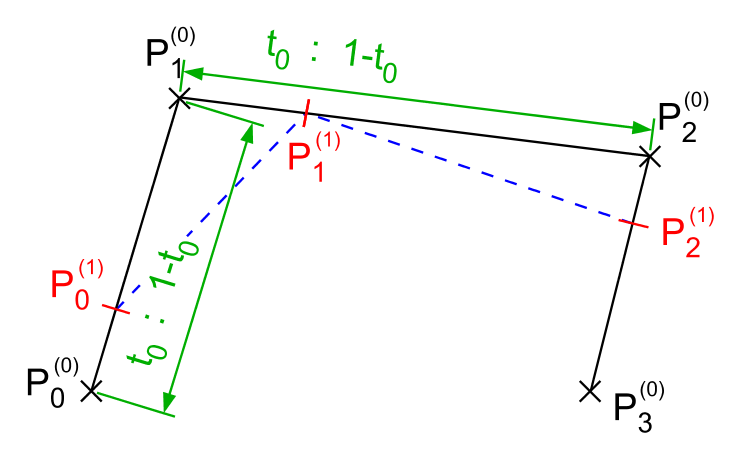
\includegraphics[width=6cm]{images/De_Casteljau_construction_1}
	    	\caption{https://commons.wikimedia.org/wiki/File:De\_Casteljau\_construction\_1.png}
        \end{figure}

        \subsection{Bézier-Splines}
        \label{kuf:sub:bezier-splines}
        
        \begin{itemize}
        	\item Bei hohem Grad beeinflusst jeder Punkt die ganze Kurve $\rightarrow$ schwierig bei Modellierung
        	\item Deshalb: Füge mehere Kurven niedrigeren Grades aneinander
        \end{itemize}
        \textbf{Definition}\\
        Stückwise polynomielle Kruve, deren einzelne Abschnitte durch Bézier-Kurven beschrieben sind
        
\end{document}
